\documentclass{article}
\usepackage[utf8]{vietnam}
\usepackage{graphicx}
\usepackage{amsmath}
\usepackage{subcaption} 

\begin{document}

\section*{1. Reproduced Table}

\begin{table}[h!]
\centering
\begin{tabular}{||c|c|c||} 
 \hline
 \textbf{Country} & \textbf{Capital City} & \textbf{Population} \\ [0.5ex] 
 \hline\hline
 Vietnam & Hà nội & 87837  \\ 
 United Kingdom & 7 & 78  \\
 United States & 545 & 778  \\
 Brazil & 545 & 18744  \\
 Columbia & 88 & 788  \\ [1ex] 
 \hline
\end{tabular}
\caption{Countries, Capital City and Population (Reproduced)}
\label{table:reproduced}
\end{table}

\section*{2. Table with Mathematical Notation}

\begin{table}[h!]
\centering
\begin{tabular}{|l|c|r|} 
 \hline
 \textbf{Indicator} & \textbf{Rate} & \textbf{Formula} \\ 
 \hline\hline
 GDP Growth (Q1) & $2.5\% \pm 0.1\%$ & $\Delta Y / Y_{t-1}$  \\ 
 Inflation (Annual) & $1.85\%$ & $\frac{P_t - P_{t-1}}{P_{t-1}} \times 100$ \\
 Pythagorean Theorem & N/A & $a^2 + b^2 = c^2$ \\
 Area of a Circle & N/A & $\pi r^2$ \\ [1ex] 
 \hline
\end{tabular}
\caption{Economic and Mathematical Notations}
\label{table:math}
\end{table}

\section*{3. Figure Demonstrating Scaling and Positioning}

\begin{figure}[h!]
    \centering
    \begin{subfigure}[b]{0.45\textwidth}
        \centering
        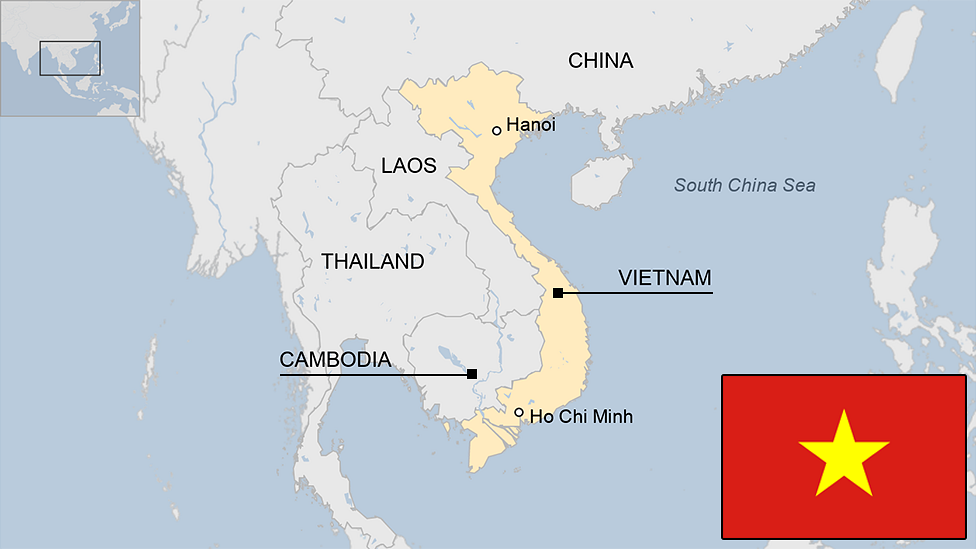
\includegraphics[width=0.4\textwidth]{vietnam.png}
        \caption{Vietnam's map (0.4\\textwidth)}
        \label{fig:vietnam_original}
    \end{subfigure}
    \hfill 
    \begin{subfigure}[b]{0.45\textwidth}
        \centering
        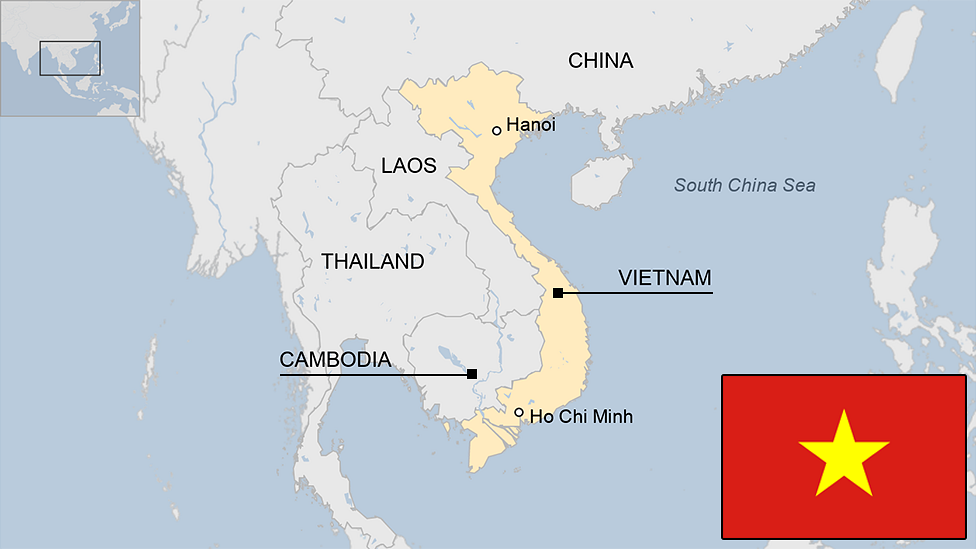
\includegraphics[width=0.5\linewidth]{vietnam.png} 
        \caption{Vietnam's map (50\% width of subfigure)}
        \label{fig:vietnam_scaled}
    \end{subfigure}
    \caption{Scaling and Positioning Example: Vietnam's map at different scales.}
    \label{figure:scaling_positioning}
\end{figure}

\end{document}